%%%%%%%%%%%%%%%%%%%%%%%%%%%%%%%%%%%%%%%%%%%%%%%%%%%%%%%%%%%%%%%%%%%%%%%%%%%%%%%%
%2345678901234567890123456789012345678901234567890123456789012345678901234567890
%        1         2         3         4         5         6         7         8
% THESIS CHAPTER

\chapter{Introduction}
\label{chap:first}
\ifpdf
    \graphicspath{{Chapter1/Figures/PNG/}{Chapter1/Figures/PDF/}{Chapter1/Figures/}{Chapter1/Figures/EPS/}}
\else
    \graphicspath{{Chapter1/Figures/EPS/}{Chapter1/Figures/}}
\fi


\section{Content}
In the introduction, please state clearly the context your work is framed within, and the motivations of your work. Furthermore, 
it is important to clarify your contribution (and not those of the group you work in - it is still an exam after all). Provide an outline of the thesis.

\section{Basic commands}
\label{sec:basic_commands}
This is a citation: \cite{cacciaActiveSonarbasedBottomfollowing1999}. Make sure to correctly enter all the bibliographic details. 
It is important that you double check them when retrieving the bibtex file from a source such as Google Scholar. Consistency in the references is valued by the Committee.

This is an emphasized word: \emph{global}.

This is a reference to another part of the thesis: Chapter \ref{chap:second}.

This is an enumerated list:
\begin{enumerate}
\item first item.
\item second item.
\end{enumerate}

This is an in-line equation: $x-$.

This is a word in quotes: ``regular''.

\section{Equation}
\label{sec:equation}

This is an equation:
\begin{equation}
{\mathcal{U}}_k(s_k) = \frac{P_k}{C_k}.
\label{eq:normal}
\end{equation}

Equations follow the punctuation rules, as if they were inline with the text.

This is an equation split over multiple lines:
\begin{equation}\label{eq:Split}
\begin{aligned}
x_{k}&={\mathcal{F}}(x_{k-1},u_{k},w_{k-1}),\\
z_{k}&={\mathcal{H}}(x_{k},v_{k}).
\end{aligned}
\end{equation}

This is an example of equation with matrices:
\begin{equation}
\mathcal{Q}_l  = \frac{{d_l ^2 \sigma _\phi  ^2 }}{2} {\begin{bmatrix}
   {2\sin ^2 \phi _l } & { - \sin 2\phi _l }  \\
   { - \sin 2\phi _l } & {2\cos ^2 \phi _l }  \\
\end{bmatrix}}
 \begin{bmatrix}{cc}
   {\frac{{\sigma _d ^2 }}{2} {\begin{array}{cc}
   {2\cos ^2 \phi _l } & {\sin 2\phi _l }  \\
   {\sin 2\phi _l } & {2\sin ^2 \phi _l }  \\
\end{array}}}  \\
\end{bmatrix}. \\
\label{eq:defQ}
\end{equation}

This is a reference to the Equation \ref{eq:Split}. Avoid using unnumbered equations as it makes it difficult to reference them during a discussion. 
Also, be consistent in the use of matrix or vector notation. 
For example, $\dot{\vec{x}}= \mat{A}\vec{x} + \mat{B}\vec{u}$ or $\vec{y} = \alpha \vec{x}$, where the $\alpha$ is a scalar. 
You can change the corresponding definitions in the class file, as long as you remain consistent.

\section{Figure}
\label{sec:figure}

I add a figure.
\begin{figure}[H]
\centering
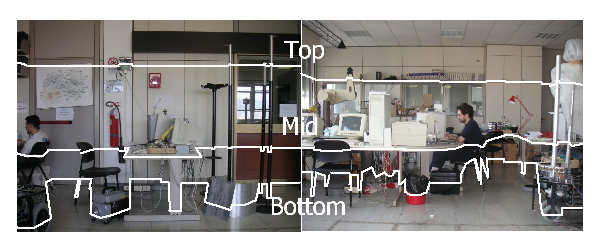
\includegraphics[width=5.0in]{Views}
\caption{Scan profiles: \emph{bottom}, \emph{mid} and \emph{top view}.}
\label{fig:views}
\end{figure}
Make sure that figures axis are readable. Make sure to label all the units on both axes. The width of the lines should 
be also crosschecked for readability (the typical MATLAB plot might need higher line width). Double check that legends are present. 
Figures' captions should allow the reader to fully understand the figure.

This is a reference to Figure \ref{fig:views}.

\section{Table}
The suggested packages for tables is tabular. There are many examples on the Internet. In general, avoid vertical lines, 
and use horizontal lines sparingly. Here S allows to align to the decimal point.
 
\begin{tabular}{SSSSSSSS} \toprule
	{$m$} & {$\Re\{\underline{\mathfrak{X}}(m)\}$} & {$-\Im\{\underline{\mathfrak{X}}(m)\}$} & {$\mathfrak{X}(m)$} & {$\frac{\mathfrak{X}(m)}{23}$} & {$A_m$} & {$\varphi(m)\ /\ ^{\circ}$} & {$\varphi_m\ /\ ^{\circ}$} \\ \midrule
	1  & 16.128 & +8.872 & 16.128 & 1.402 & 1.373 & -146.6 & -137.6 \\
	2  & 3.442  & -2.509 & 3.442  & 0.299 & 0.343 & 133.2  & 152.4  \\
	3  & 1.826  & -0.363 & 1.826  & 0.159 & 0.119 & 168.5  & -161.1 \\
	4  & 0.993  & -0.429 & 0.993  & 0.086 & 0.08  & 25.6   & 90     \\ \midrule
	5  & 1.29   & +0.099 & 1.29   & 0.112 & 0.097 & -175.6 & -114.7 \\
	6  & 0.483  & -0.183 & 0.483  & 0.042 & 0.063 & 22.3   & 122.5  \\
	7  & 0.766  & -0.475 & 0.766  & 0.067 & 0.039 & 141.6  & -122   \\
	8  & 0.624  & +0.365 & 0.624  & 0.054 & 0.04  & -35.7  & 90     \\ \midrule
	9  & 0.641  & -0.466 & 0.641  & 0.056 & 0.045 & 133.3  & -106.3 \\
	10 & 0.45   & +0.421 & 0.45   & 0.039 & 0.034 & -69.4  & 110.9  \\
	11 & 0.598  & -0.597 & 0.598  & 0.052 & 0.025 & 92.3   & -109.3 \\ \bottomrule
\end{tabular}
\section{Algorithm} 
\label{sec:algorithm}

This is an algorithm:
\begin{algorithm}[H]
\label{alg:SMS}
\caption{Split \& Merge [\& Split]}
\begin{algorithmic} [1]
\REQUIRE{A scan $s$. A stack $\mathcal{L}$. A counter $j$. A threshold $\tau$}
\ENSURE{$\lambda \leftarrow \mathcal{M}(s)$, $j=1, ..., |\lambda|$}
\STATE{$\mathcal{L}$ = \texttt{push}($s$)}
\STATE{$j \leftarrow 1$}
\WHILE{$\mathcal{L}$ $\neq$ $\varnothing$}
\STATE{$\mathcal{L}$ = \texttt{pop}($s_{top}$)}
\STATE{$l_j$ $\leftarrow$ \texttt{fitting}($s_{top}$)}
\STATE{$q_k = \argmax_{q}\texttt{dist(l$_j$,q)}$}
\IF{$\texttt{dist(l$_j$,$q_k$)} < \tau$}
\STATE{$j \leftarrow j+1$}
\STATE{\texttt{continue}}
\ELSE
\STATE{$s_a \leftarrow$ \texttt{sub}($s_{top}$, 1, $k$)}
\STATE{$s_b \leftarrow$ \texttt{sub}($s_{top}$, $k+1$, $|s|$)}
\STATE{$\mathcal{L}$ = \texttt{push}($s_a$)}
\STATE{$\mathcal{L}$ = \texttt{push}($s_b$)}
\ENDIF
\ENDWHILE
\STATE{\{$l_j$\} $\leftarrow$ \texttt{merge}(\{$l_j$\})}
\STATE{\{$l_j$\} $\leftarrow$ \texttt{split}(\{$l_j$\})}
\end{algorithmic}
\end{algorithm}

% NOMI DA RIDEFINIRE

\section{Historical background}
% parlare della curiosità uomo legata a fondale del mare (allargare)
% parlare delle criticità legate all'ambiente marino
The first real underwater explorations date back to the Phoenicians, Greeks, and Romans, who, through diving and free diving, recovered corals, sponges, and objects from the seabed, in addition to defenses \cite{erodotoStorieVsec.a.C.}.
Many years later, in 1535, Guglielmo de Lorena designed the first underwater bell for underwater inspections, but only at shallow depths \cite{eliavGuglielmosSecretEnigma2015}.
It was not until 1934 that the first real exploratory expedition took place with William Beebe and Otis Barton's bathyscaphe to a depth of about 923 meters, and in 1960, Auguste Piccard's bathyscaphe, the Trieste, reached a depth of 10,916 meters in the Mariana Trench \cite{jacquespiccardSevenMiles1961}.

% approfondire questione navigazione trieste

% Concentrarsi su evoluzione sensori  per veicoli marini guidati da uomo
% Concentrarsi su esplorazioni con uomo dentro veicolo marino su fondale

\subsection{Marine robotics}
%  % Passaggio ai ROV e motivazione della scelta
With the advent of technology, remotely operated vehicles (ROVs) emerged, allowing for deeper and more complex underwater exploration without putting human divers at risk. The most complex challenge was the communication between the ROV and the surface vessels. The solution was to build tethered systems that could maintain a constant connection.
The CURV, Cable Controlled Undersea Recovery Vehicle, was the first ROV to be used in underwater missions.
% Storia breve dei ROV
% Descrivere svantaggi ROV risolvibili con AUV storici

% % Passaggio agli AUV
% Storia AUV
% Motivarli e dare i pregi che hanno portato al nuovo sviluppo

\subsection{Autonomous navigation}
% Storia Sistemi di navigaazione AUV
% Storia Sensoristica AUV per navigazione
\subsection{Underwater mission in seabed inspection}
% Storia Missioni per esplorazione di barriere coralline e fondali piu recenti e complessi

\section{Motivation}
% Motivare l'importanza della navigazione autonoma negli AUV e l'impiego degli AUV in generale
\section{Problem statement}
% definire i problemi legati agli attuali sistemi di navigazione AUV attraverso descrizione dei problemi dei paper

\section{Previous work and main contribution} % ARGOMENTO PRINCIPALE TERRAIN TRACKING
% Creare lo stato dell'arte recente del mio ambito -> illustare possibili scelte e lavori precedenti simili ai miei mostrando possibili criticità
% - Spiegare architettura blocchi degli AUV, estraendo componenti e andando su TT
% - Importance of Terrain Tracking
% - Problems with Terrain Tracking
% - Possible solutions for Terrain Tracking
% RIVEDERE TUTTI I POSSIBILI PUNTI NELLO STATO DELL'ARTE
\subsection{Terrain tracking types} % possibili esterne soluzioni
\subsection{EKF and echosonar usage}
\subsection{Sensors in AUV} % non so se metterlo

\section{Thesis outline}
% Creazione di una breve descrizione di ogni capitolo
\emph{Chapter} \ref{chap:second} 

\emph{Chapter} \ref{chap:third} 

\emph{Chapter} \ref{chap:fourth} 

\emph{Chapter} \ref{chap:fifth} 

\emph{Chapter} \ref{chap:sixth} 

\emph{Chapter} \ref{chap:seventh} 

\emph{Chapter} \ref{chap:results} 
% Fare alla fine
% Scaletta logica con i passaggi importanti di ogni capitolo molto brevemente